\documentclass[../main.tex]{subfiles}
\graphicspath{{\subfix{../Images/}}}
\begin{document}

%\section{Perception Geometry} \label{perception_geometry}

Minion is equipped with six \ac{LiDAR} sensors as well as six cameras to perceive her surroundings.
Omnidirectional \ac{LiDAR} coverage is provided by three Velodyne VLP-16 units for situational awareness within the \acp{USV} immediate operating environment.
% \ac{LiDAR} coverage and object detection within the vessel's immediate operating environment.
Three additional forward-scanning Livox Horizon \ac{LiDAR} units generate a dense point cloud ahead of the vessel for object detection and classification at greater distances.
The Livox units are directly mounted to a camera enclosure which houses four high-definition visual-spectrum cameras and two \ac{LWIR} cameras.
The combination of forward-scanning LiDAR and cameras provides a significantly higher fidelity of data within a shared 165-degree \ac{FOV}. % in the direction of travel.
% The camera enclosure design emphasizes modularity and research flexibility.
Figure~\ref{fig:camera_enclosure} illustrates the mounting arrangement of the Livox Horizon LiDAR units and the six cameras within the waterproof enclosure.
Together, these sensors define the operational envelope of the perception system, encompassing a horizontal \ac{FOV} of approximately 160~degrees and an effective detection range of up to 60~meters.

\begin{figure}[htbp]
\centering
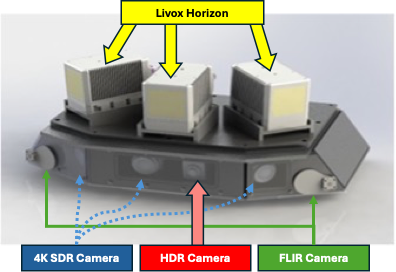
\includegraphics[width=0.6\textwidth]{Images/Camera_enclosure2.png}
\caption{Mounting locations of three Livox Horizon LiDAR units (yellow arrow, top), two LWIR cameras (green, thin, solid arrows), three FLIR 4k cameras (blue, dotted arrows), and a single \ac{HDR} camera  (red arrow, bottom) within the camera enclosure.}
\label{fig:camera_enclosure}
\end{figure}

% While the Velodyne \ac{LiDAR} sensors provide comprehensive 360-degree environmental awareness for navigation and collision avoidance, the three forward-facing Livox Horizon \ac{LiDAR} units mounted to the camera enclosure were selected for their superior point cloud density and ability to facilitate a higher resolution for object detection.
% The three Livox units concentrate sampling density in the forward \ac{FOV}, matching the horizontal coverage of the six cameras.
% Both modalities overlap the \ac{FOV} of their respective individual sensors.
% This sensor arrangement ensures higher density and more uniform point-cloud across the 165-degree forward perception envelope in the case of \ac{LiDAR}, but also makes the system more robust to failure.
% Losing a single sensor will not create a blind spot for either sensing modality in the forward path of motion of the \ac{USV}. 
% Figures~\ref{fig:fov_cam} and ~\ref{fig:fov_LiDAR} show how the horizontal \ac{FOV} for each of these sensors overlaps in the direction of travel.

% Each of these sensors is installed so that the center of their \ac{FOV} is parallel to one of three separate lines of vision.
% The first of these lines is a vector that points down the centerline of the vessel in the forward direction, and sensors in this orientation receive the moniker of \texttt{sensor\_center}.
% The other two lines of vision are rotated 40 degrees counterclockwise and clockwise from the centerline, and sensors in these orientations receive the moniker \texttt{sensor\_port} and \texttt{sensor\_starboard}, respectively.
Each sensor’s optical axis is aligned with one of three predefined sight lines: the vessel's centerline and two axes rotated $\pm 40$ degrees from the center.
% In the case of LiDAR, this sensor arrangement provides a denser point cloud and, in general, means that the loss of signal from any single sensor does not create a blind spot in the forward direction of travel.
For the LiDAR system, this configuration increases point-cloud density in the forward direction and ensures that loss of any single sensor does not produce a blind spot in the forward direction of travel.
% Figure~\ref{fig:fov_combined} shows the camera's \ac{FOV} in \ref{fig:fov_cam}, and the the LiDAR \ac{FOV} in \ref{fig:fov_LiDAR}.
Each of the three Livox Horizon LiDAR units has an 81.7-degree \ac{FOV}, resulting in more than a 40-degree overlap in the \ac{FOV} between \texttt{livox\_center} and both \texttt{livox\_port} and \texttt{livox\_starboard}, and approximately 3 degrees of overlap between \texttt{livox\_port} and \texttt{livox\_starboard} (figure~\ref{fig:fov_LiDAR}).
Three 4K cameras are configured to point in along each of these three sight lines. 
While these cameras are equipped with a Theia-TL410P zoom lens, they are currently set at a fixed zoom level that approximates a 65-degree horizontal \ac{FOV}, which provides a 15-degree overlap in their \ac{FOV} (figure~\ref{fig:fov_cam}).
The two \ac{LWIR} cameras each have a 90-degree \acs{FOV}, and are positioned along the port and starboard vision lines, providing a 10-degree overlap.
Finally, there is a single HDR camera with a 65-degree horizontal \ac{FOV} that points forward.
While the \ac{HDR} camera lacks any of the aforementioned sensor redundancy, its \ac{FOV} aligns with the central 4k camera and was added for research that compared the two center-line mounted cameras \cite{liebergall}.

% related to the dynamic range of the two center-line mounted cameras  and was selected as the primary visual range sensor for this body of work for reasons that are discussed in section~\ref{visual_cameras}.


\begin{figure}[htbp]
\centering
\begin{subfigure}[t]{0.48\textwidth}
    \centering
    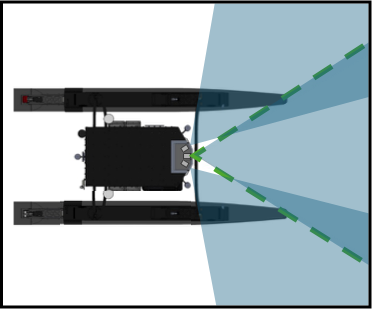
\includegraphics[width=\textwidth]{Images/fov_cam.png}
    \caption{Blue cones represent \ac{FOV} from individual FLIR 4K camera; green dashed lines indicate \ac{FOV} of HDR camera.}
    \label{fig:fov_cam}
\end{subfigure}
\hfill
\begin{subfigure}[t]{0.48\textwidth}
    \centering
    \includegraphics[width=\textwidth]{Images/fov_LiDAR.png}
    \caption{LiDAR horizontal \ac{FOV} overlap.}
    \label{fig:fov_LiDAR}
\end{subfigure}
\caption{Comparative visualization of horizontal \ac{FOV} (FOV) overlap for (a) cameras and (b) LiDAR sensors.}
\label{fig:fov_combined}
\end{figure}

% A Torc Robotics PinPoint \ac{GPS}/\ac{IMU} system is equipped with provides both global time synchronization and platform pose estimation.

% The sensor coordinate frames are organized in a hierarchical transformation tree structure, which is shown in \ref{transform_diagm}.
% The inertial reference frame (\texttt{map}) defines the world-fixed coordinate system.
% The platform reference frame (\texttt{base\_link}) represents the vessel body frame defined by the PinPoint \ac{GPS}/\ac{IMU}.
% The center Livox frame (\texttt{livox\_center}) serves as the primary sensor reference frame, with \texttt{livox\_port} and \texttt{livox\_starboard} both reporting data in the \texttt{livox\_center} reference frame.
% Six camera image frames exist within this tree, and are referenced to the \texttt{livox\_center} frame.
% Intrinsic calibration parameters, including camera-specific matrices and distortion coefficients, along with extrinsic transformation parameters relating sensor frames to each other and to the platform frame, are discussed in \textcolor{red}{Appendix \#}.

% The Livox scan pattern employs a non-repetitive rosette pattern that progressively covers the \ac{FOV} over time rather than repeatedly sampling fixed positions.
% This characteristic enables temporal aggregation to increase effective spatial resolution, particularly beneficial for a moving platform where \ac{GPS}/\ac{IMU} pose data enables motion-compensated point cloud accumulation.

% The dual \ac{LiDAR} architecture serves complementary purposes.
% The Velodyne VLP-16 units provide the omnidirectional awareness required for autonomous navigation, while the Livox Horizon sensors optimize point cloud density specifically within the forward camera \ac{FOV} for fusion research.
% The onboard This configuration enables comparative evaluation of detection performance while maintaining operational navigation capabilities.
% The sensor suite supports the research objectives of comparing detection performance across modalities and evaluating late fusion approaches.
% The following subsections detail individual sensor specifications and selection rationale.

% The primary sensors used for the data collected for this research were from the forward-facing perception module, referred to as the camera enclosure.

%%%%%%%%%%%%%%%%%%%%%%%%%%%%%%%%%%%%%%%%%%%%%%%%%%%%%%%%%%%%%%%%%%%%
%%%%%%%%%%%%%%%%%%%%%%%%%%%%%%%%%%%%%%%%%%%%%%%%%%%%%%%%%%%%%%%%%%%%

\end{document}
